\section{Так квинтовый или квартовый? Квинто-квартовый круг}
\label{ch:harmony:kvinto-kvarto-round}

На самом деле полное название этого полезного помощника, которого легко сделать из бумаги: <<квинто-квартовый круг мажорных и минорных тональностей>>. Выглядит он странно: см. рисунок \ref{fig:harmony:kvinto-kvarto:kvinto-kvarto-final}. И хотелось бы не только научиться им пользоваться, но и понять почему он именно такой.

Круг может помочь, если вы хотите:
\begin{itemize}
    \item Подобрать <<сочетающиеся>> аккорды для аккомпанемента песен.
    
    \item Определить, какие ноты входят в ту или иную мажорную или минорную тональность.
    
    \item Сменить <<тональность>> аккомпанемента песни. Человеческим языком: \emph{каждую} ноту исходной тональности нужно повысить или понизить на заданное количество полутонов. Зачем? Чтобы было удобнее петь. При этом интервальная структура (т.е. характер, например, веселый или грустный) музыки не изменится, а произведение <<в целом>> будет звучать ниже или выше, <<подстраиваясь>> таким образом под голос исполнителя.    

    \item Решить <<академические>> задачки, например, определить тональность произведения по нотам или определить параллельную тональность.
    
    \item Найти закономерности в ваших удачных музыкальных импровизациях.
    
    \item И много чего ещё\ldots
\end{itemize}

Мы не будем сейчас учиться как решать эти задачки, мы начнем разбираться с устройством круга. В процессе станет понятно не только, как решать эти задачки, но и много чего ещё\ldots

Глядя на рисунок \ref{fig:harmony:interval:octave-kon-dis} можно увидеть, что для отдельно взятого звука в пределах октавы существует лишь \emph{два} звука, образующий с исходным звуком совершенный консонанс. Относительно исходного эти звуки находятся на расстоянии в 5(\myNemph{кварта}) и 7(\myNemph{квинта}) полутонов. Оказывается, что можно переупорядочить ноты так, чтобы совершенные консонансы стали соседями исходного звука: один справа, другой слева!

Начнём, например с ноты ДО, и отступая по семь полутонов по часовой стрелке:
\[
    C\rightarrow 
    G\rightarrow 
    D\rightarrow 
    A\rightarrow 
    E\rightarrow 
    B\rightarrow 
    {F\sharp}\rightarrow
    {C\sharp}\rightarrow
    {G\sharp}\rightarrow
    {D\sharp}\rightarrow
    {A\sharp}\rightarrow
    F\rightarrow 
    C,
\]
замкнем круг и получим результат, представленный на рисунке \ref{fig:harmony:kvinto-kvarto:kons-rearrange}.

\begin{figure}[!ht]
    \centering
    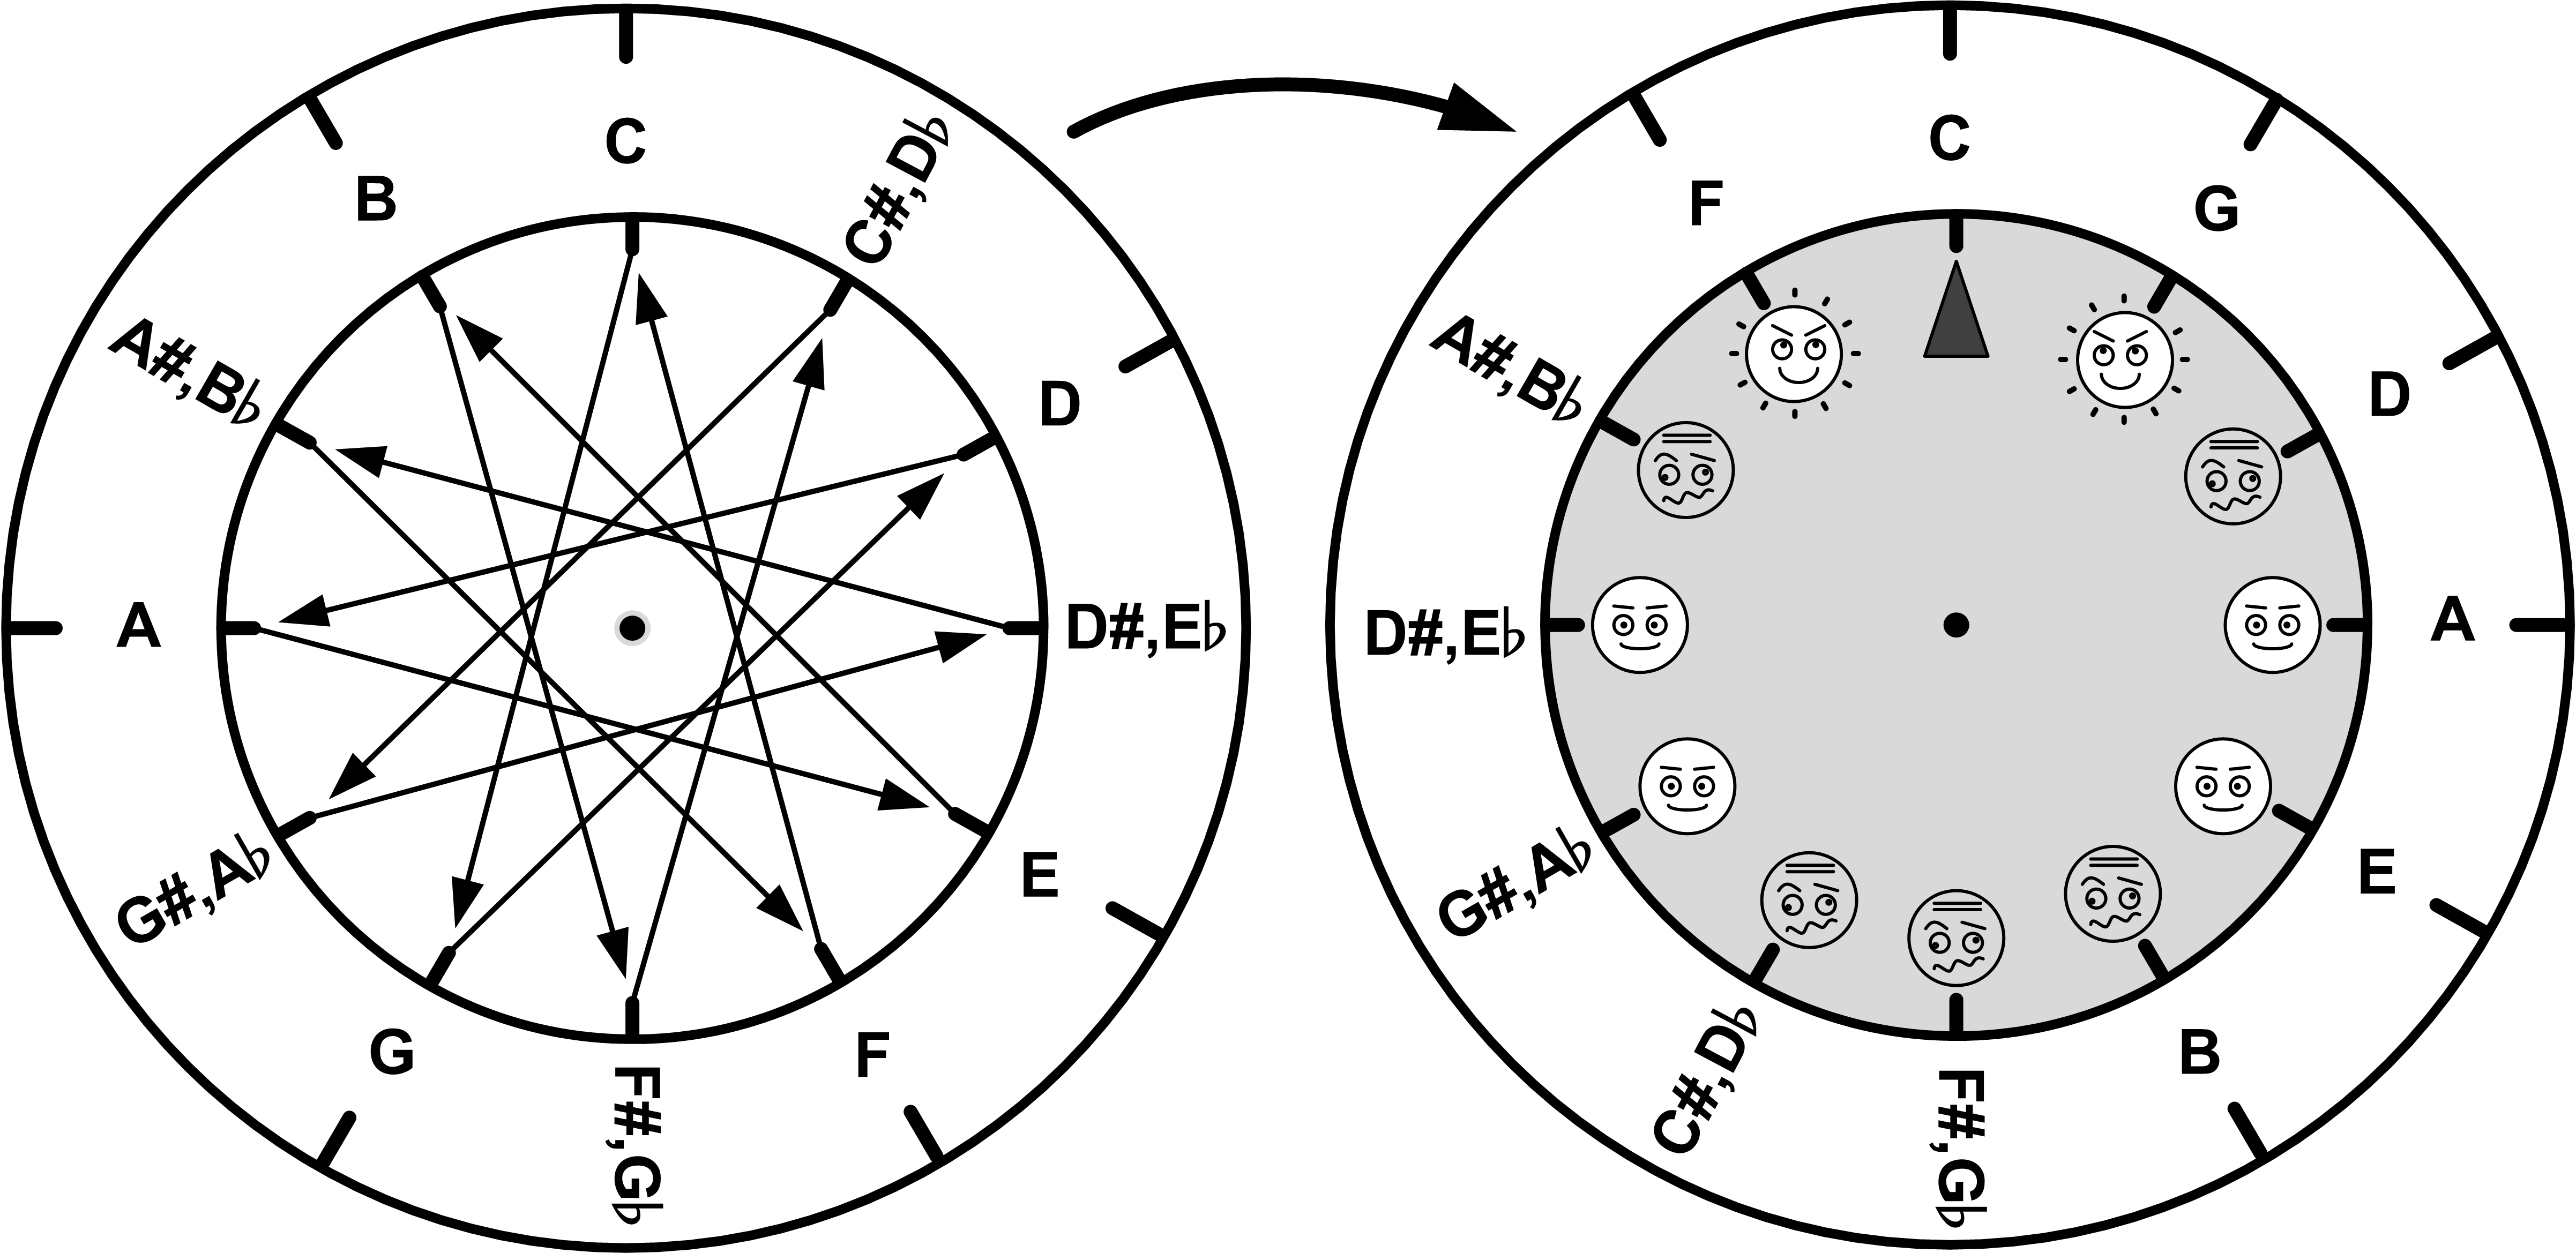
\includegraphics[scale=0.7]{fig/kvinto-kvarto/kons-rearrange} 
    \caption{Консонансы по соседству}\label{fig:harmony:kvinto-kvarto:kons-rearrange}
\end{figure} 

Теперь достаточно ткнуть в любую ноту на получившемся круге и узнать её совершенные консонансы: соседом против часовой стрелки будет совершенный консонанс на расстоянии 5 полутонов (чистая кварта), а по часовой --- консонанс на расстоянии 7 полутонов (чистая квинта). Например, возмьем ноту ЛЯ(A) и сразу определяем консонансы: РЕ(D) --- кварта от ЛЯ и МИ(E) --- квинта.

Обратите внимание на то, что среди переупорядоченных нот явно выделились две цепочки: цепочка нот без диезов и бемолей и цепочка нот со знаками альтерации. Конечно, это не случайность: ноты без диезов и бемолей --- это названия ступеней мажорного лада (а точнее --- тональность ДО-мажор). И само-собой, мажорный лад в своё время был сформирован с учетом расположения совершенных консонансов и вполне возможно, автор при этом глядел на полученный нами круг.

Итак, ноты тональности ДО-мажор (т.е. ноты без знаков альтерации) выстроились на полученном круге в одну цепочку. При этом тоника --- ДО, идет в этой последовательности второй, если считать по часовой стрелке.

Таким образом упростилась задача определения нот для \emph{любой} мажорной тональности: 
\begin{enumerate}
    \item нужно отметить тонику на круге и отступить от нее на один сектор против часовой стрелки;
    \item включая полученную ноту, двигаясь по часовой стрелке, отсчитать семь нот тональности.
\end{enumerate}

Например, требуется определить ноты тональности РЕ-мажор (см. рисунок \ref{fig:harmony:kvinto-kvarto:d-maj}). Отступаем от $D$ против часовой стрелки, а затем по часовой собираем 7 нот:
\[
    G\rightarrow 
    D\rightarrow 
    A\rightarrow 
    E\rightarrow 
    B\rightarrow 
    {F\sharp}\rightarrow
    {C\sharp}
\]

\begin{figure}[!ht]
    \centering
    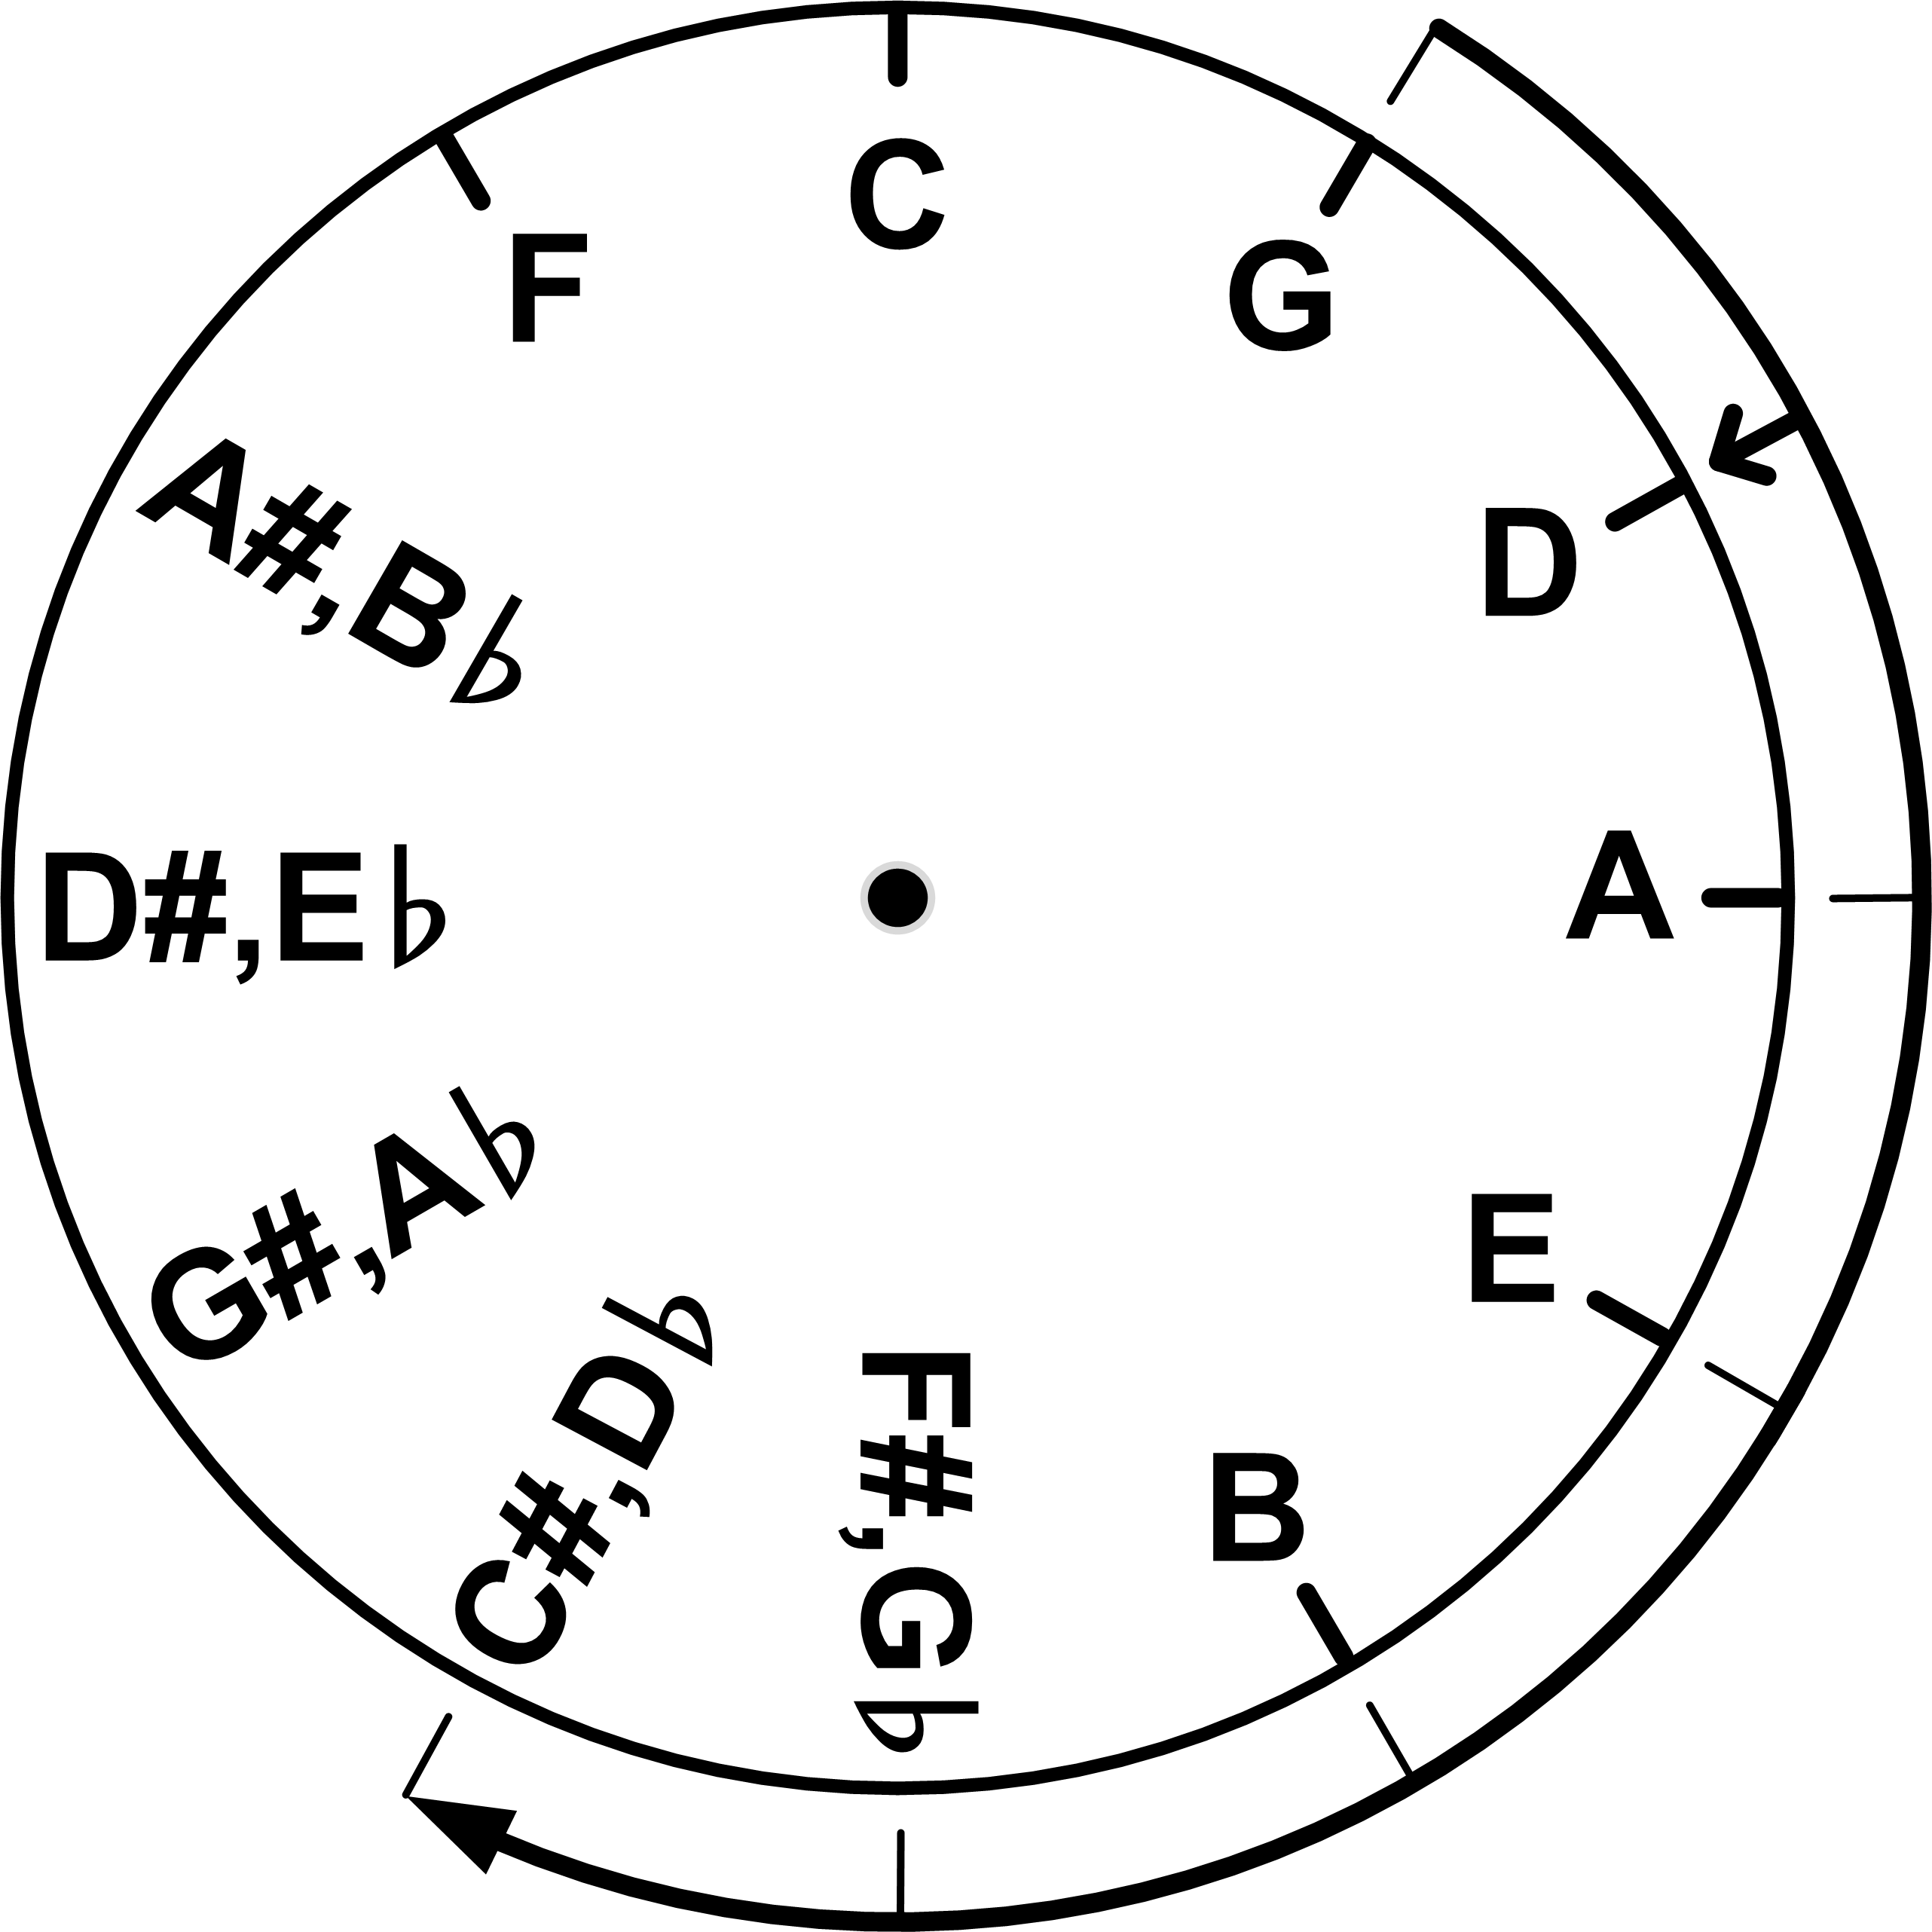
\includegraphics[scale=0.5]{fig/kvinto-kvarto/kvinto-kvarto-d-maj} 
    \caption{Ноты тональности $D$-maj}\label{fig:harmony:kvinto-kvarto:d-maj}
\end{figure}

Естественно, что ноты по высоте пока не упорядочены, но это совсем несложно сделать, зная, что тоника <<внизу>>:
\[
    D\rightarrow 
    E\rightarrow 
    {F\sharp}\rightarrow
    G\rightarrow 
    A\rightarrow 
    B\rightarrow 
    {C\sharp}
\]

Мы разобрались, как определять ноты любой мажорной тональности. И мы уже знаем, что для любой мажорной тональности можно подобрать <<параллельную>> ей минорную тональность\footnote{Для тональности любого диатонического лада можно подобрать <<параллельную>> тональность из другого диатонического лада}. Напомню, что параллельные тональности состоят из одних и тех же нот, но отличаются тоникой --- самым низким звуком. Поэтому музыкальные звуки, соответствующие одинаковым нотам параллельных тональностей, могут иметь разное высотное положение, то есть находиться в разных октавах.

Мажорный и минорный лады --- фундамент музыки. Особенно они востребованы при составлении аккомпанемента к песням. Поэтому ограничиться шпаргалкой только для мажорного лада никак нельзя: нужно подключить и минорный\footnote{Кто внимательно читал раздел \ref{ch:harmony:lad}, тот знает, что, например, тональность ЛЯ-минор параллельна тональности ДО-мажор. Таким образом, отличие лишь в том, что тоника ЛЯ будет находится в последовательности нот без знаков альтерации (ДО-мажор) пятой по счету по часовой стрелке. Так что по имеющемуся на данный момент круге уже можно определить ноты и для любой минорной тональности: отступаем пять секторов от тоники против часовой стрелки и собираем семь нот --- по часовой}.

Возьмем три круга (см. рисунок \ref{fig:harmony:kvinto-kvarto:minor-major-mapping}), и разобъем каждый их них на 12 равных секторов. На первом (самом большом) круге отметим 12 нот в их естественной последовательности; на втором (поменьше, на рисунке \ref{fig:harmony:kvinto-kvarto:minor-major-mapping} выделен серым цветом) --- отметим ступени мажорного лада; на третьем (самом маленьком) --- ступени минорного. Насадим все круги на общую ось, проходящую через центр каждого круга.

\begin{figure}[!ht]
    \centering
    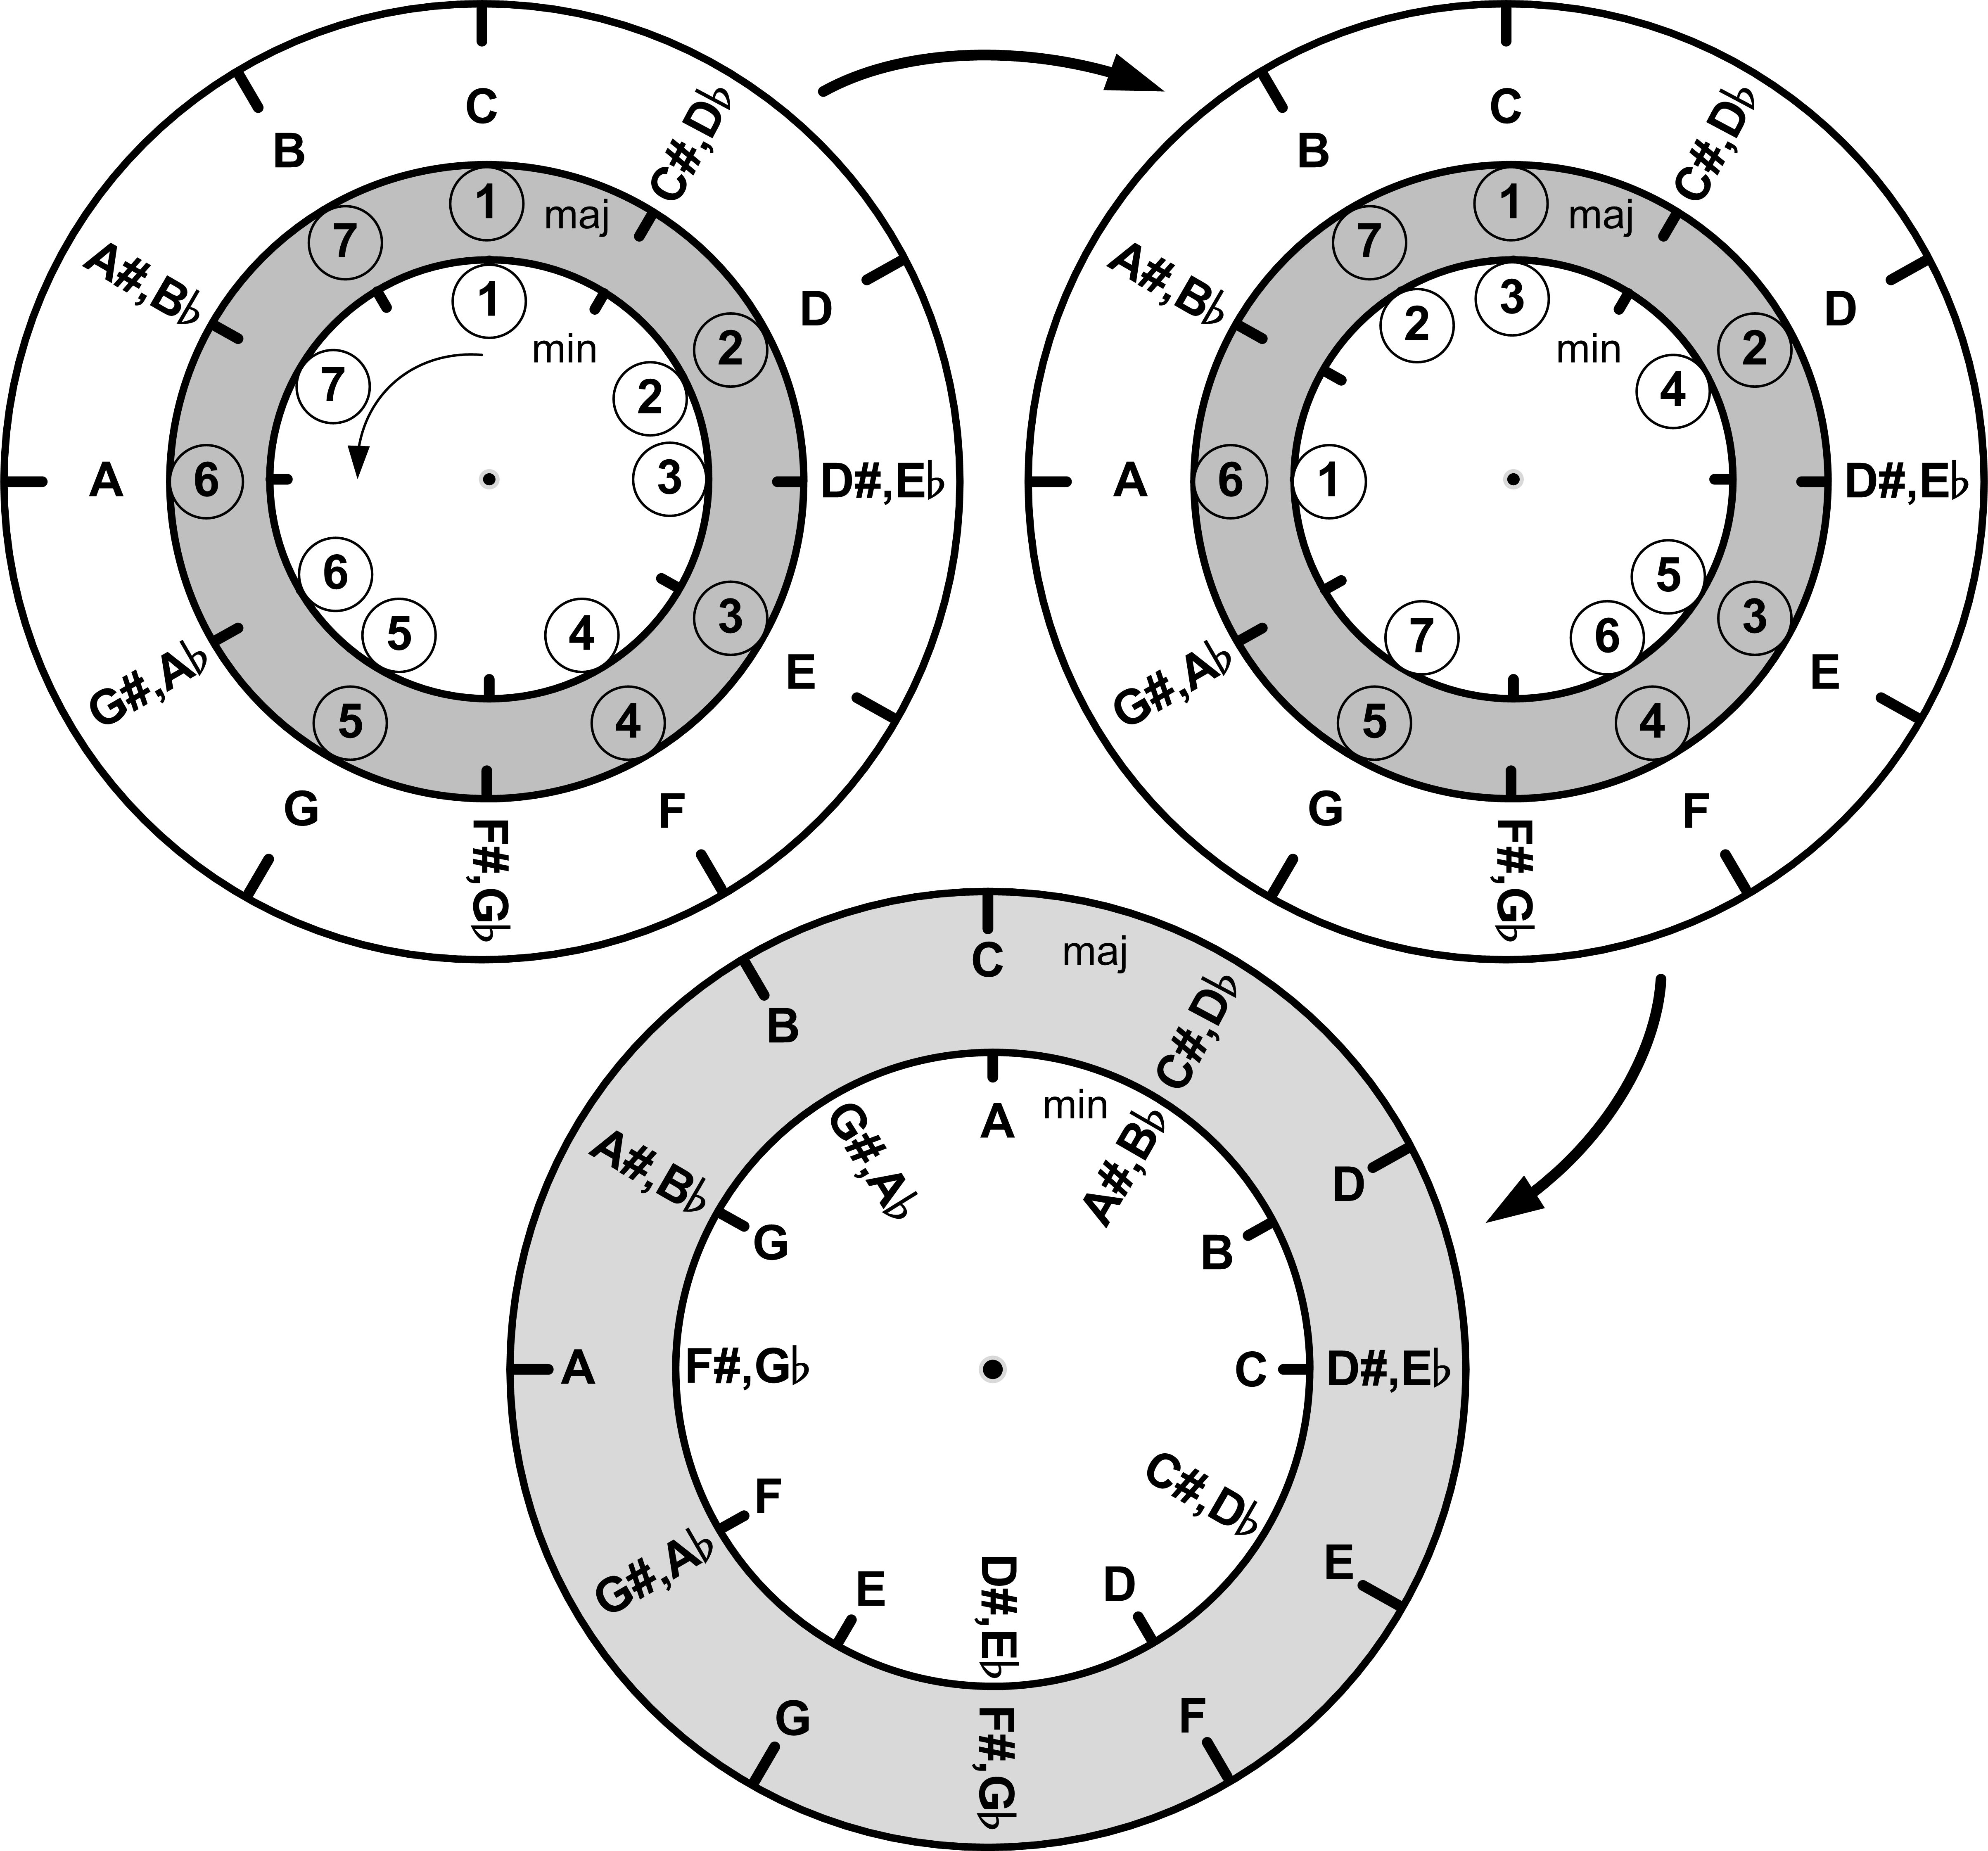
\includegraphics[scale=0.5]{fig/kvinto-kvarto/minor-major-mapping} 
    \caption{Соответствие тоник параллельных мажорных и минорных тональностей}\label{fig:harmony:kvinto-kvarto:minor-major-mapping}
\end{figure}

Если на получившемся приборе совместить шестую ступень мажорного лада с первой ступенью минорного лада (ну или первую ступень мажора с третьей ступенью минора), то будет видно, что они имеют сходную интервальную структуру и порождают параллельные тональности, т.е. тональности, в которые входят одинаковые ноты. Зафиксируем в таком положении кружки со ступенями и будем проворачивать круг с нотами. На рисунке \ref{fig:harmony:kvinto-kvarto:minor-major-mapping} показана ситуация, когда первая ступень мажора указывает на тонику ДО(C), а первая ступень минора --- на тонику ЛЯ(A). ДО-мажор и ЛЯ-минор --- параллельные тональности. Видно, что на внешнем круге с нотами, тоника параллельной минорной тональности находится на расстоянии трех секторов против часовой стрелки от соответствующей тоники мажорной тональности. Полное соответствие тоник параллельных мажорных и минорных тональностей представлено на рисунке \ref{fig:harmony:kvinto-kvarto:minor-major-mapping}.

Вернемся к нашей <<квинто-квартовой>> перестановке нот и выпишем для неё (во внутренней части круга) тоники параллельных минорных тональностей. Получим предварительный вариант круга, представленный на рисунке \ref{fig:harmony:kvinto-kvarto:kvinto-kvarto-parallel}.

\begin{figure}[!ht]
    \centering
    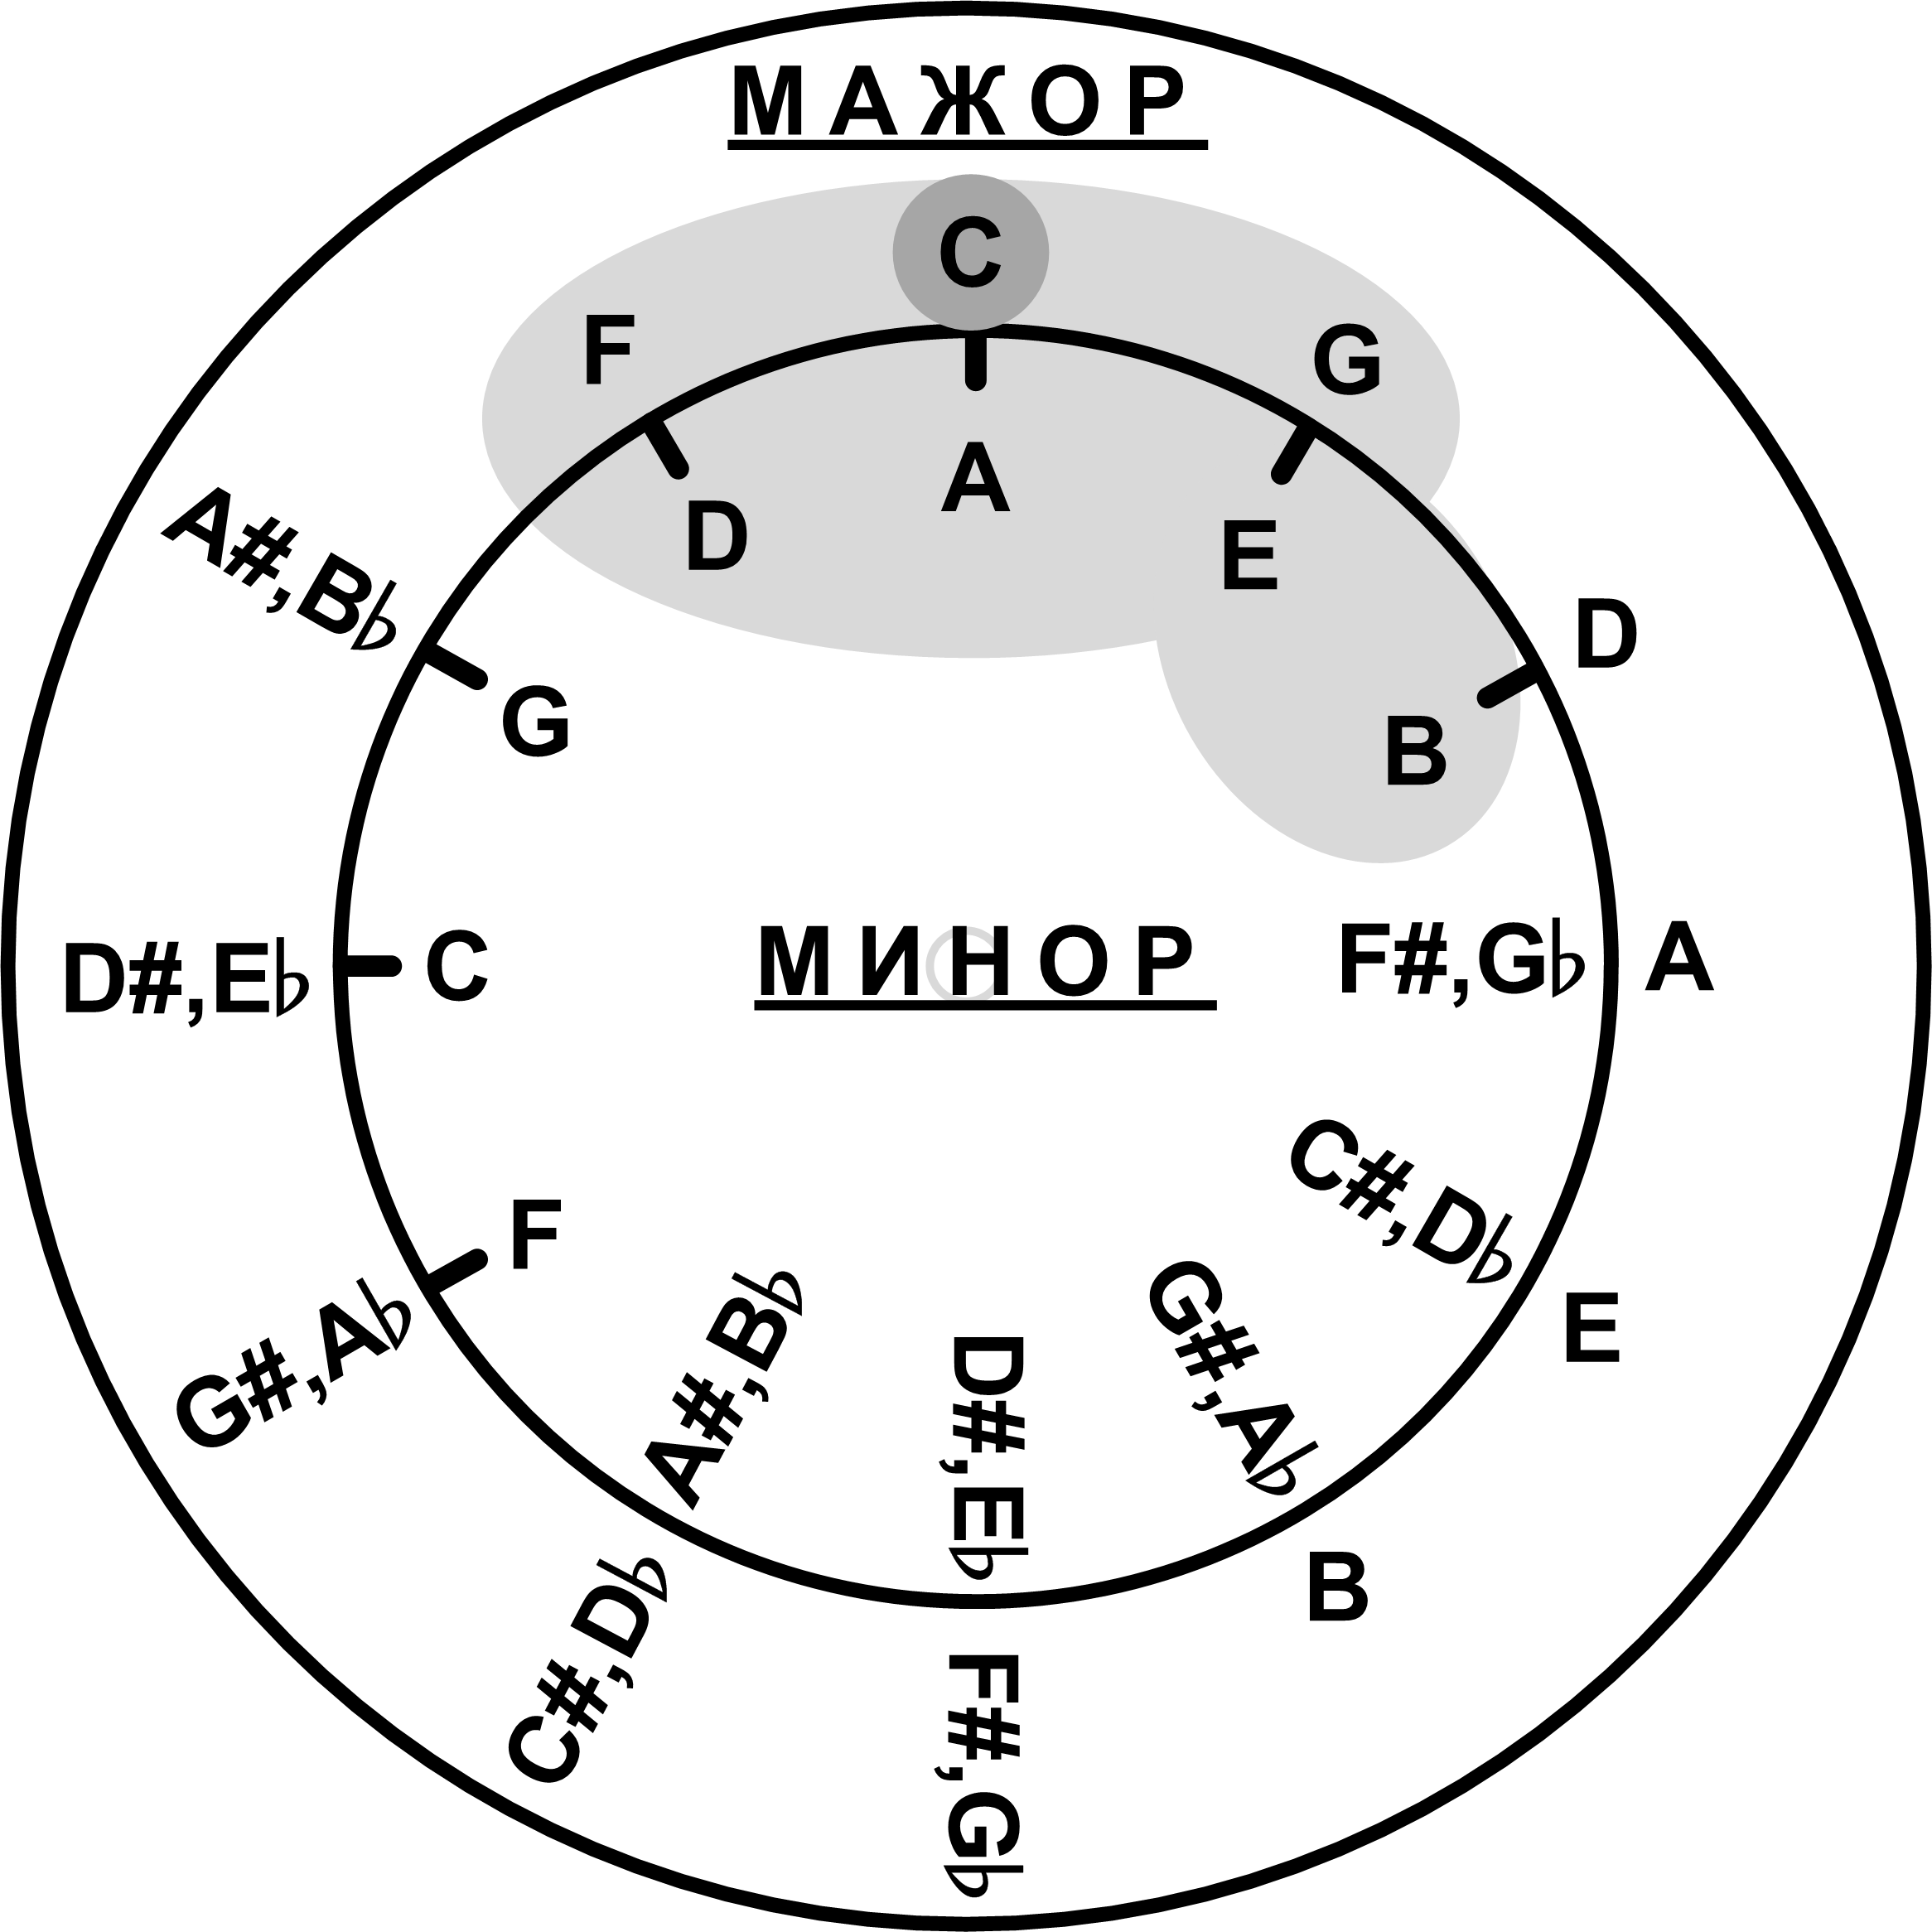
\includegraphics[scale=0.5]{fig/kvinto-kvarto/kvinto-kvarto-parallel} 
    \caption{Квинто-квартовый круг параллельных минорных и мажорных тональностей (базовая версия)}\label{fig:harmony:kvinto-kvarto:kvinto-kvarto-parallel}
\end{figure}

Если приглядеться к рисунку \ref{fig:harmony:kvinto-kvarto:kvinto-kvarto-parallel} внимательнее, то можно увидеть, что внутренний круг нот (параллельные минорные тоники) просто повёрнут на три сектора против часовой стрелки относительно мажорных тоник. Так как и на внутреннем (минорнм), так и на внешнем (мажорном) круге одни и те же ноты идут в одном и том же порядке (они только смещены друг относительно друга), то ноты мажорной тональности стало ещё проще искать. Например, ноты тональности ДО-мажор выделены на рисунке \ref{fig:harmony:kvinto-kvarto:kvinto-kvarto-parallel} серым цветом. Вам лишь нужно найти мажорную тонику (в примере --- ДО(C), выделена более темным оттенком серого) на внешнем круге и выделить группу соседних нот, а также парных им на <<минорном>> круге, ну и останется добавить еще одну нотку, являющуюся соседкой выделенной группе на минорном круге (по часовой стрелке, в примере ей оказаласт нота СИ(B)).

Ноты минорной тональности найти так же просто: нужно найти тонику на внутреннем, минорном, круге, а затем отметить соответствующую ей тонику мажорной тональности. Всё. Дальше те же действия, что и для поиска нот мажорной тональности\footnote{Когда и если будете упорядочивать ноты минорной тональности по высоте не забудьте взять тонику именно минорной тональности}.

Круг в принципе готов и им уже можно пользоваться, но давайте поможем и академическим кругам! Эти бедняги часто сталкиваются с подобной задачкой. Дано:

\begin{center}    
    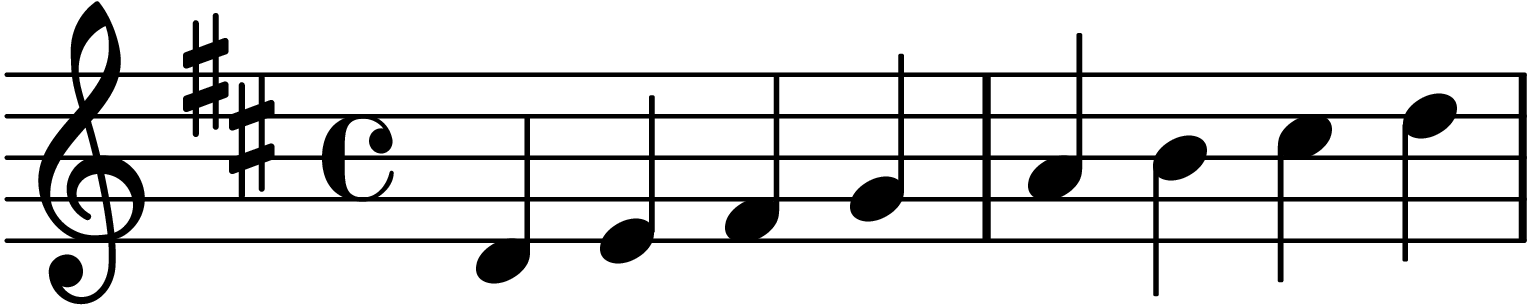
\includegraphics{fig/kvinto-kvarto/tonality-d-maj}
\end{center}

Найти: мажорную тональность, в которой записана <<музыка>>, ориентируясь на знаки альтерации после скрипичного ключа.

Конечно, можно напрячься и определить, что <<под диезом>> находятся ноты ФА(F) и ДО(C). Находим их на мажорном круге. Остальные ноты, стало быть без знаков альтерации, они появятся в последовательности, только в том случае, если двигаться от ФА-диез по мажорному кругу против часовой стрелки (и их пять). Мажорная тоника, как мы помним, вторая по счету в последовательности: значит это РЕ(D). Тональность РЕ-мажор!

Как говорила Ба в серии рассказов <<Манюня>> Наринэ Абгарян: 
\begin{center}
    <<Господибожетымой!!!>>
\end{center}

Ну или как-то так\ldots Лады, конечно, ладами, но в какой же кошмар они превращают чтение нот!

Чтобы хоть немного упростить себе жизнь, музыканты \emph{договорились} определять тональность по типу и количеству знаков альтерации, встретившихся после ключа. При этом пришлось пойти на некоторые <<технические>> ухищрения. Давайте рассмотрим их на финальной версии круга, изображенной на рисунке \ref{fig:harmony:kvinto-kvarto:kvinto-kvarto-final}.

\begin{figure}[!ht]
    \centering
    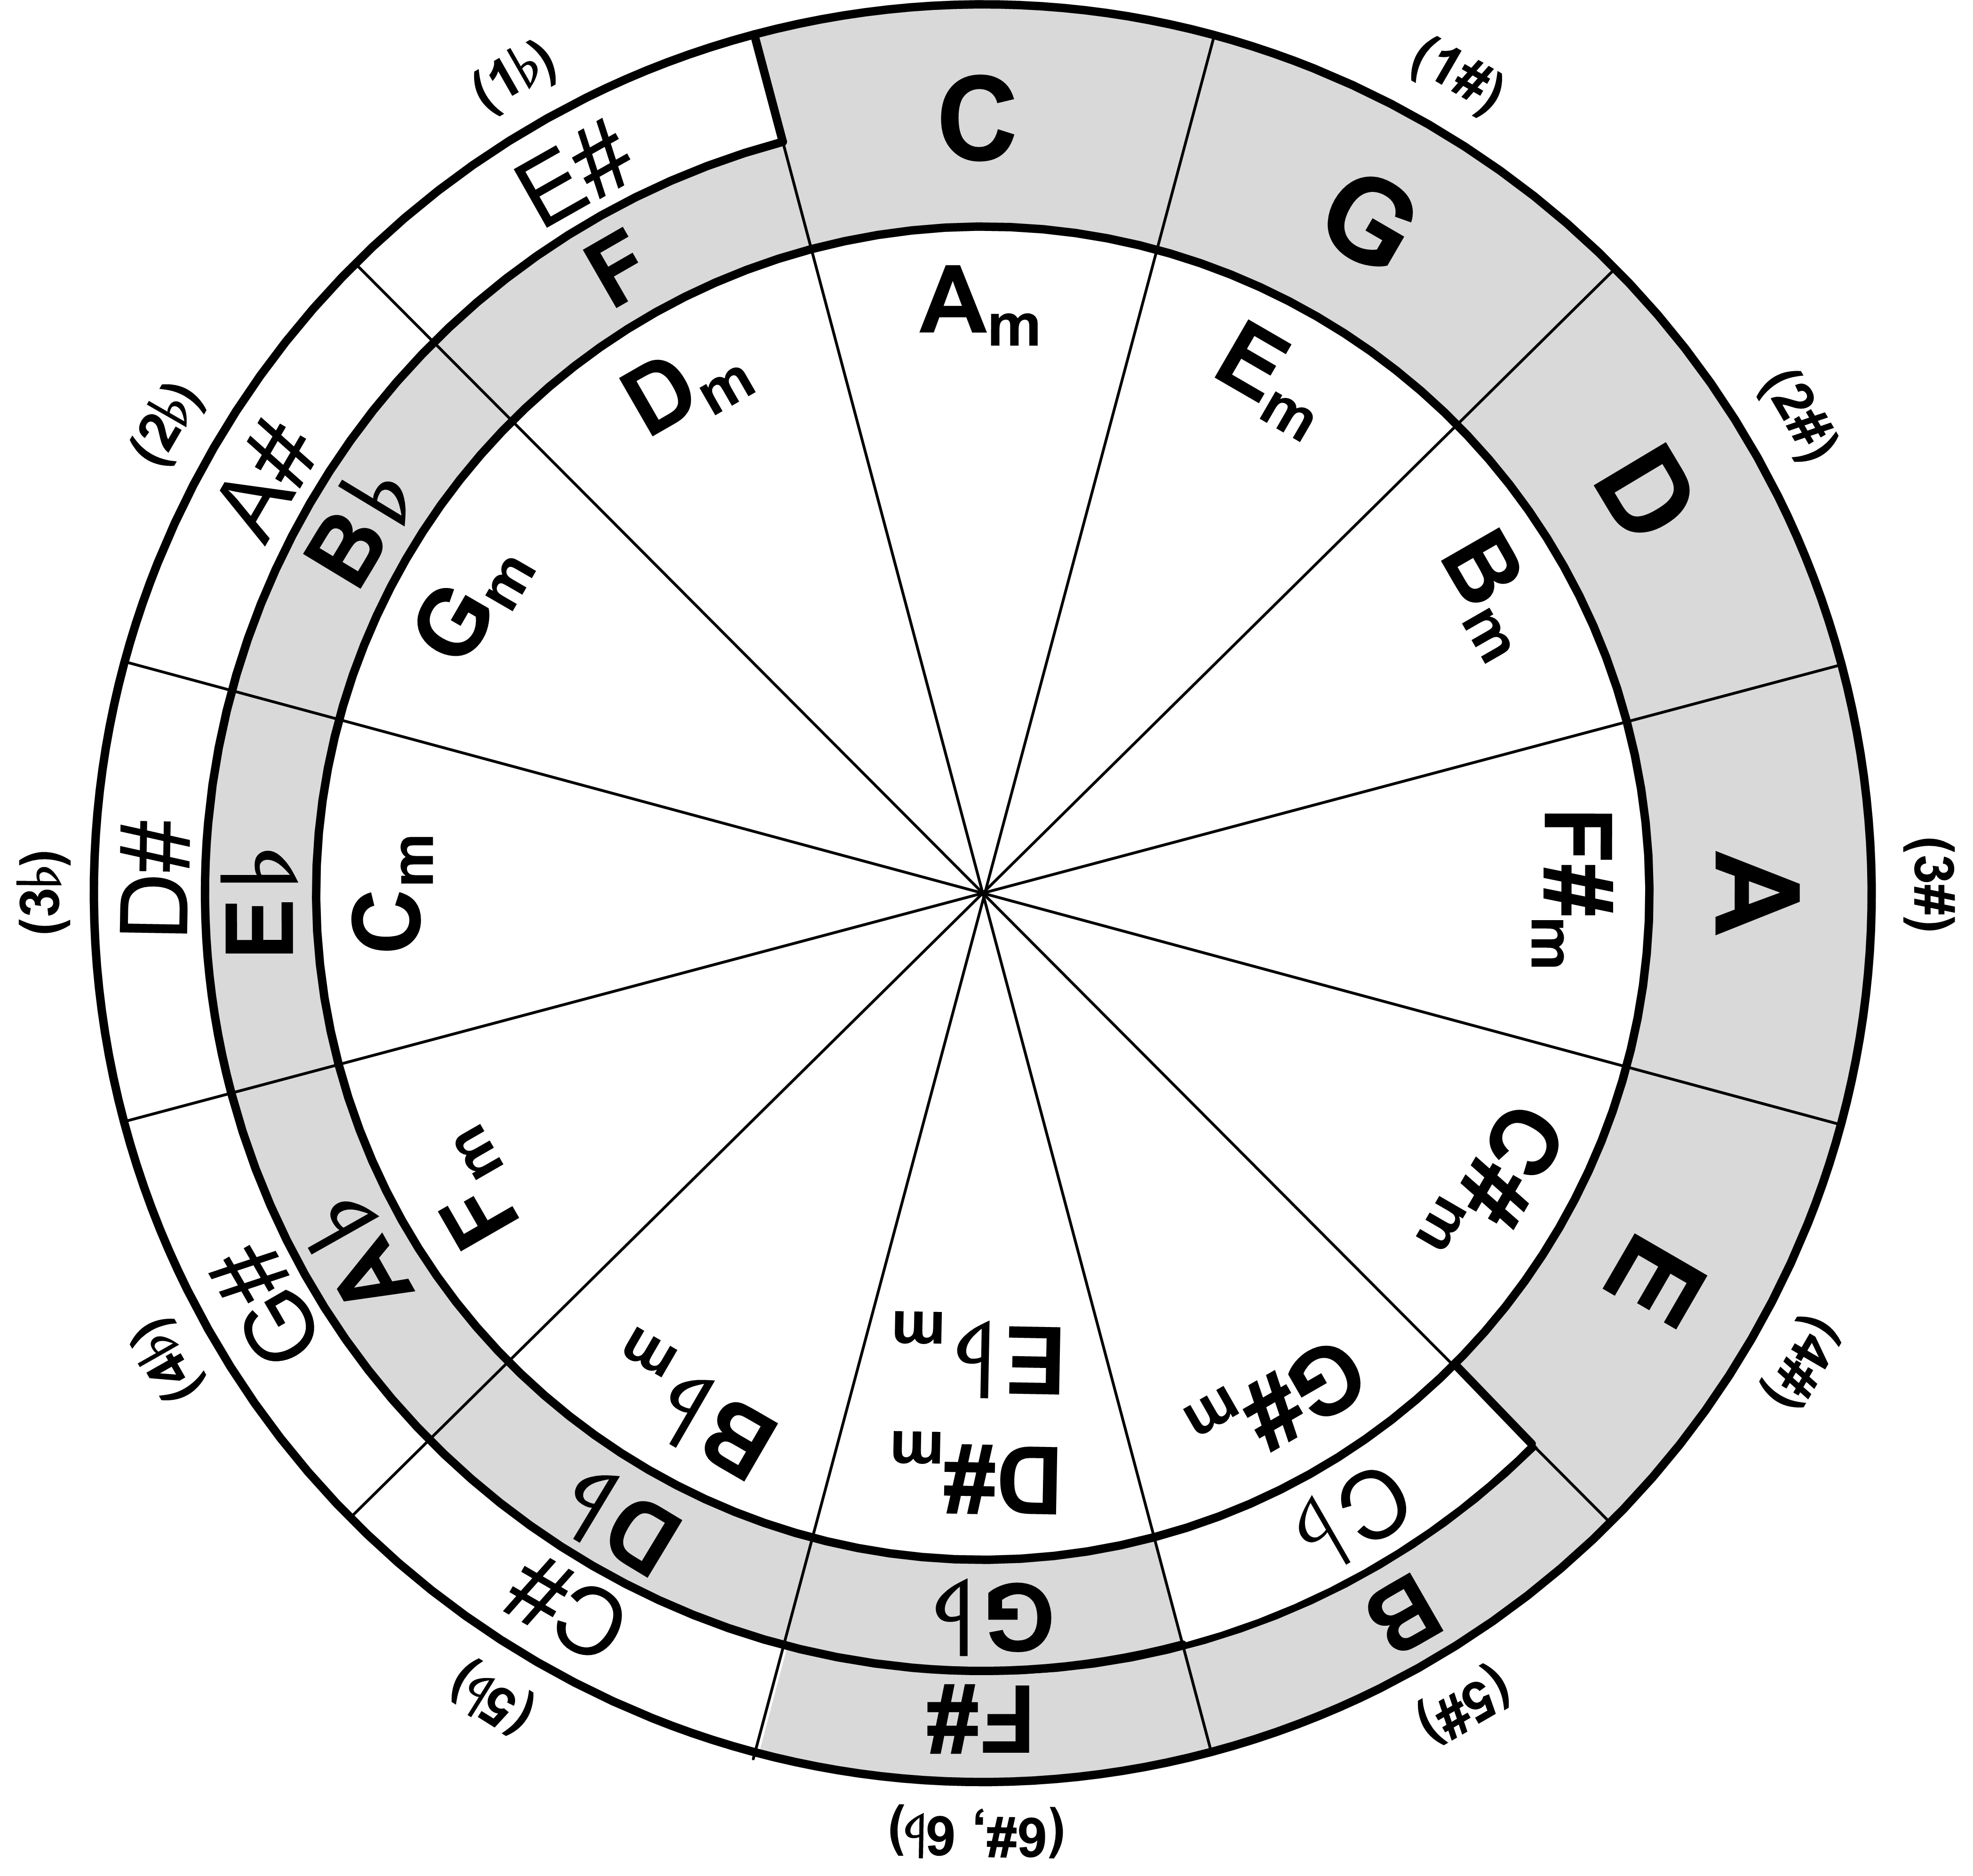
\includegraphics[scale=0.8]{fig/kvinto-kvarto/kvinto-kvarto-final} 
    \caption{Квинто-квартовый круг мажорных и минорных тональностей\index{круг квинто-квартовый}}\label{fig:harmony:kvinto-kvarto:kvinto-kvarto-final}
\end{figure}

Отметим, что ноты мажорных тональностей образуют теперь своеобразную спираль: 
\begin{itemize}
    \item эта спираль начинает <<наматываться>> по часовой стрелке с ноты ДО-бемоль ($C\flat$);
    
    \item далее следует привычная группа альтерированных нот, но при этом используется только знак альтерации бемоль ($\flat$):
    \[
        {G\flat}\rightarrow
        {D\flat}\rightarrow
        {A\flat}\rightarrow
        {E\flat}\rightarrow
        {B\flat};
    \]
    
    \item виток продолжается группой нот без знаков альтерации:
    \[
        F\rightarrow
        C\rightarrow
        G\rightarrow
        D\rightarrow
        A\rightarrow
        E\rightarrow
        B;
    \]
    
    \item далее опять начинается привычная группа альтерированных, но теперь только знаком диез ($\sharp$) нот, идущих как бы вторым слоем по аналогичным, альтерированным ранее бемолем ($\flat$) нотам: 
    \[
        {F\sharp}\rightarrow
        {C\sharp}\rightarrow
        {G\sharp}\rightarrow
        {D\sharp}\rightarrow
        {A\sharp}\rightarrow
        {E\sharp}.
    \]
\end{itemize}

Стоит также обратить внимание, что на круге (рисунок \ref{fig:harmony:kvinto-kvarto:kvinto-kvarto-final}) появились <<странные>> ноты $E\sharp$ и $C\flat$. Они нужны, чтобы увеличить количество нот с соотвествующим знаком альтерации до шести, ведь в противном случае по количеству знаков альтерации некоторые тональности различить бы не удалось. Представьте, что например, мы не ввели бы для ноты СИ($B$) её альтерированный аналог ДО-бемоль($C\flat$). Тогда для тональности СОЛЬ-бемоль-мажор $C\flat$-maj мы получили бы набор с пятью альтерированными нотами:
\[
    B\rightarrow
    {G\flat}\rightarrow
    {D\flat}\rightarrow
    {A\flat}\rightarrow
    {E\flat}\rightarrow
    {B\flat}\rightarrow
    F.
\]

Но тогда и тональность РЕ-бемоль-мажор($D\flat$):
\[
    {G\flat}\rightarrow
    {D\flat}\rightarrow
    {A\flat}\rightarrow
    {E\flat}\rightarrow
    {B\flat}\rightarrow
    F\rightarrow
    C
\]
имела бы те же самые пять альтерированных нот, что и ДО-бемоль-мажор: по числу знаков альтерации их бы различить не удалось. А вот с нововведением ДО-бемоль($C\flat$) вместо СИ($B$), тональность СОЛЬ-бемоль-мажор разживется шестью знаками альтерации и спутать её с другой тональностью будет уже невозможно:
\[
    {C\flat}\rightarrow
    {G\flat}\rightarrow
    {D\flat}\rightarrow
    {A\flat}\rightarrow
    {E\flat}\rightarrow
    {B\flat}\rightarrow
    F.
\]

Ту же сказку можно рассказать и о <<рождении>> МИ-диез ($E\sharp$).

Теперь обратите внимание на пометки количества тех или иных знаков альтерации, идущих по внешней границе круга (в скобках). Они просто выписаны заранее, чтобы не собирать ноты тональности обычным образом и не пересчитывать ноты со знаками альтерации.  

Теперь, если вы увидели нечто подобное:

\begin{center}    
    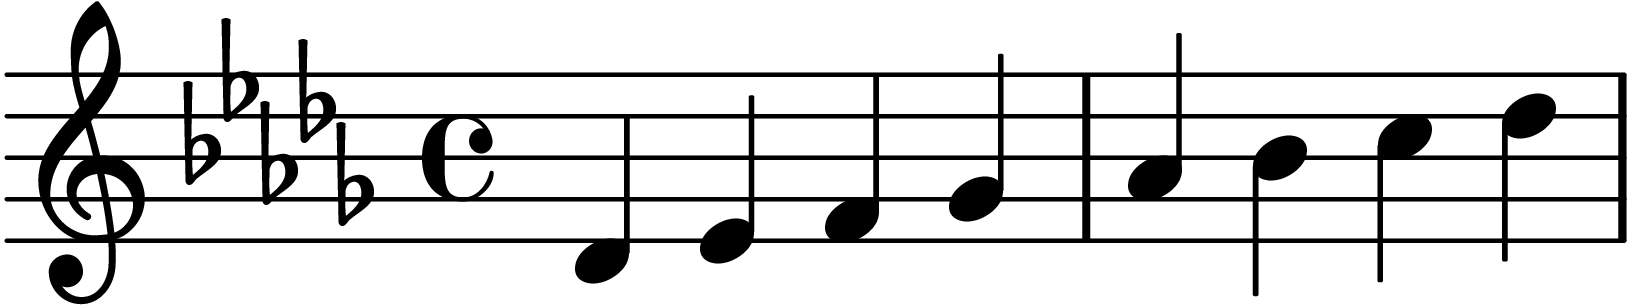
\includegraphics{fig/kvinto-kvarto/tonality-des-maj}
\end{center}

то вам достаточно лишь посчитать количество бемолей и сразу определить, что вы имеете дело с тональностью РЕ-бемоль-мажор($D\flat$-maj), или может быть с параллельной ей СИ-бемоль-минор($B\flat$-min)\ldots

Закрепим:
\begin{center}    
    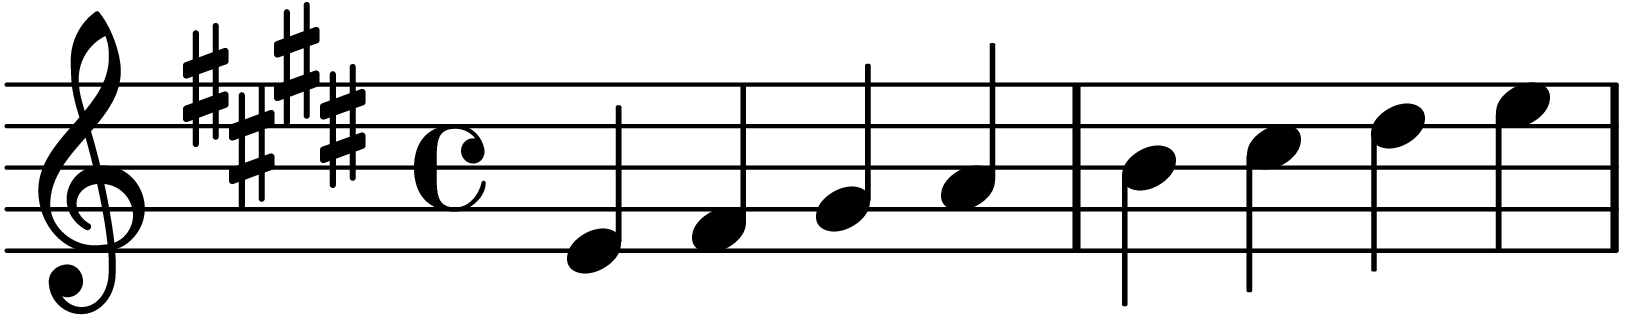
\includegraphics{fig/kvinto-kvarto/tonality-e-maj}
\end{center}
ну да, МИ-мажор($E$-maj) или ДО-диез-минор($C\sharp$-min).

Серым цветом на <<мажорной спирали>> выделены ноты, которые \emph{принято} использовать в качестве тоник мажорных тональностей. Правильно сказать <<ЛЯ-бемоль-мажор>> ($A\flat$-maj), а вот <<СОЛЬ-диез-мажор>> ($G\sharp$-maj) --- уже нарушение этикета, хотя вроде бы полностью эквивалентные вещи. Скажете так на музыкальной конференции --- и кто-то из слабых сердцем профессоров может уйти в мир иной от такого невежества. Для обозначения параллельных минорных тоник также используются не все ноты.

Заметили, что для обозначения минорных тоник, используется индекс <<$m$>>? Теперь исходные обозначения нот (тоник) стали очень похожи на обозначения аккордов. Это неспроста: с помощью круга действительно подбирают аккорды для аккомпанемента авторских песен. Например, в песне <<Звезда по имени солнце>> используются аккорды: $A_m$, $C$, $D_m$, $G$. Найдите их на круге и поразмышляйте о тональности этой песни.
